\documentclass[../thesis.tex]{subfiles}
\begin{document}
	\section{Experimental Environment}
	\subsection{Local Server Environment}
	The local servers are setup using the three different web technologies, namely Node, PHP and Django. Each of the servers are able to run simultaneously on the same machine on different ports. Below is the setup and configuration for each of the servers. The servers are setup using the http server module that comes bundled with each of the web technologies. 
	\newline
	
	In order to keep the readings consistent, the local servers are setup on the same machine and are connected to the same network. The operating system on the local server machines is Windows 10, CPU speed 2.6 GHz and 16 GB RAM.
	\subsection*{Node Server}
	In order to setup the Node server, the following pre-requisites are required - 

	\begin{itemize}
		\item NPM - Node package manager
		\item Node
		\item Express framework
	\end{itemize}

	Node package manager gives us access to open-source packages that aid in the development of Node applications. It comes bundled with the installation of Node.
	\newline

	Once we choose a folder in which the server files will reside, we run the terminal and execute the following command - `npm install express`
	\newline

	This installs the express middleware framework that provides us with the necessary modules to develop a Node server. After the installation completes we observe a folder structure as follows - 
	\begin{verbatim}
	|-node_modules
	|-src
	|---index.html
	|---index.js
	|-package.json
	\end{verbatim}
	The node\_modules folder contains all the necessary packages that express requires, some of the notable packages are the 'http-server', 'babel' etc. Te src files contains all the server related files, index.html is the homepage of the server that is returned when a request is made to the server. index.js is where the server code lives. The simplest method to fire a web server using Node and express is shown below - 
	\begin{verbatim}
	var express = require('express');
	var app = express();
	
	app.get("/*", (req, res) => {
	res.sendFile(path.join(__dirname, "index.html"));
	});
	
	app.listen(9000, () => console.log("Running on 9000"));
	\end{verbatim}
	The above code fires a server that runs on localhost port 9000. When a request is made to the home page http://localhost:9000/ ('/' indicates homepage) the server receives the request and the \lstinline|app.get("/")| function fires and sends a response with index.html file.
	\newline

	index.html is a simple static HTML file that gets served as the homepage when a request is made. Depending on the server and application the homepage can be configured as required.
	\begin{verbatim}
	<!DOCTYPE html>
	<html lang="en">
	
	<head>
	<meta charset="UTF-8">
	<meta name="viewport" content="width=device-width, initial-scale=1.0">
	<meta http-equiv="X-UA-Compatible" content="ie=edge">
	<title>Document</title>
	</head>
	
	<body>
	<h1>This is API file</h1>
	</body>
	
	</html>
	\end{verbatim}
	The homepage here simply displays the title 'This is API file' on the browser when a request is made for it.
	\newline

	The package.json file is where the configurations for the server and dependencies are configured. For the purpose of this project we have utilized the following dependencies - "cors", "express", "pg" these are application specific dependencies.
	\newline

	\begin{itemize}
		\item \textbf{cors} is a package that enables cross-origin resource sharing, which makes use of additional HTTP headers in order to let a user gain permission of resources that are on a different server, in our case to gain access to resources in the remote server configuration.

		\item \textbf{express} as discussed previously, is a Node.js framework for server configuration.

		\item \textbf{pg} is the package that enables connection to the postgreSQL database.
	\end{itemize}

	Additionally, Node also supports packages that are only used in the development phase, they are listed under the devDependencies object, some of the important devDependencies used in this project are - 
	\bigskip
	\begin{itemize}
		\item \textbf{body-parser} is a middleware which parses the incoming request's body header in req.body property.

		\item \textbf{babel-cli} used for compilation of different Javascript files written in the latest ECMAScript 6 in order to transpile them to ECMAScript 5 which is understandable by the browsers.

		\item \textbf{nodemon} watches the server files for any changes and restarts the server automatically when changes are made, hence it gets rid of the manual restarting of the server needed to be done by the developer.
	\end{itemize}

	The server is fired by running the script in the scripts object present in the package.json file.
	\begin{verbatim}
	"scripts": {
	"start": "nodemon --exec babel-node -- src/index.js"
	},
	\end{verbatim}
	nodemon is set to watch the index.js file which is where our server code lives and updates the server if any changes are made to this file. babel-node executes the ECMAScript 6 code in index.js and transpiles it to ECMAScript 5 which is understandable to the web browser. When the server is ready we get the following message in the console if everything worked - 
	\begin{verbatim}
	[nodemon] 1.12.1
	[nodemon] to restart at any time, enter 'rs'
	[nodemon] watching: *.*
	[nodemon] starting 'babel-node src/index.js'
	Running on 9000
	\end{verbatim}
	Therefore the server is now running and listening to requests on port 9000.
	
	\subsection*{PHP Server}
	Local PHP servers can be set up relatively easily in comparison to the other two web technologies considered in this project. XAMPP for Windows makes setting up a local server on the machine relatively easy. It provides a WAMP stack (Windows, Apache, MySQL and PHP). The steps involved in setting up a PHP server are as follows -
	\newline

	\begin{itemize}
		\item \textbf{Creating Virtual Hosts}
		\newline

		There are a number of ways to serve static PHP files from the server. One way is to simply keep all server related files within the 'htdocs' folder in XAMPP. However, the drawback of this is that we have to enter long URLs for every page that we want to visit. Instead we can create a virtual host for each of our sites which have different URLs. The virtual hosts set up is located in the following file: 
		\begin{verbatim}
		/xampp/apache/conf/extra/httpd-vhost.conf
		\end{verbatim}
		At the bottom of the file append the following:
		\begin{verbatim}
		NameVirtualHost 127.0.0.1:80
		
		<VirtualHost 127.0.0.1:80>
		DocumentRoot "C:/xampp/htdocs/"
		ServerName localhost
		</VirtualHost>
		\end{verbatim}
		This sets the root of localhost to 'C:/xampp/htdocs'. So all the server calls made to localhost will look for the url in this folder. 
		\smallskip
		\item Now all we have to do is run the XAMPP control panel and start the Apache server. This fires the PHP server on port 80 and serves the PHP files located inside the 'C:/xampp/htdocs' folder. If we navigate to 'http://localhost/' in our web browser, the server returns the index.php file since it is the homepage. The xampp/htdocs/ folder structure is as follows - 
		\begin{verbatim}
		|-img
		|-xampp
		|-index.php
		|-favicon.ico
		\end{verbatim}
		The 'img' folder contains all the static images that are used by the web application, favicon.ico is the icon that is visible on the title bar of the browser when we navigate to the website. index.php is the homepage of the website and is returned when a request is made from the browser.
	\end{itemize}
	
	\subsection*{Django Server}
	Django is extremely versatile in terms of how it can be installed and configured. Django can be: 
	\newline

	\begin{itemize}
		\item Installed from source, PyPi (Python Package Index) or by using package manager applications in UNIX operating systems.
		\smallskip
		\item Installed on various operating systems.
		\smallskip
		\item Configured to use several of the popular databases.
		\smallskip
		\item Run within a Python virtual environment or within the system environment.
	\end{itemize}
	In order to install and setup Django, we need the following -

	\begin{itemize}
		\item \textbf{Python} - The Python version used in this project is version 3.6
		\smallskip
		\item \textbf{pip} - Python package manager used to install Django.
	\end{itemize}
	Once we have these two requirements fulfilled, we simply need to install Django. It is done in the command prompt (on Windows) or terminal (on Linux) by running the following command -
	\begin{verbatim}
	pip install django
	\end{verbatim}
	The django version used in this project is 2.0.2.
	Once everything is installed, we need to create our server, this is done in the terminal by running - 
	\begin{verbatim}
	django-admin startproject projectname
	\end{verbatim}
	Where project name is the name of the project. This creates a folder with the name provided as the projectname, with the following structure:
	\begin{verbatim}
	|-projectname
	|---settings.py
	|---urls.py
	|-applicationname
	|---migrations
	|---views.py
	|---urls.py
	|---models.py
	|-manage.py
	\end{verbatim}
	The manage.py is the main file through which the server is built. It puts our project's package into the sys.path and also sets the DJANGO\_SETTINGS\_MODULE environment variable to make it point to our project's settings configuration file.
	\begin{verbatim}
	#!/usr/bin/env python
	import os
	import sys
	
	if __name__ == "__main__":
	os.environ.setdefault("DJANGO_SETTINGS_MODULE", "projectname.settings")
	try:
	from django.core.management import execute_from_command_line
	try:
	import django
	execute_from_command_line(sys.argv)
	
	\end{verbatim}
	The projectname/settings.py file contains all the configurations for our server, such as database settings, application specific settings, middleware configurations, template routing, authentication handlers etc. projectname/urls.py manages the routing of the website. The `urlpatterns` list routes URLs to views.
	\begin{verbatim}
	from django.conf.urls import include, url
	from django.contrib import admin
	
	urlpatterns = [
	url(r'^admin/', admin.site.urls),
	url(r'^$', include('fibonacci.urls')),
	url(r'^api/fibonacci/', include('fibonacci.urls')),
	url(r'^api/books/', include('books.urls'))
	]	
	\end{verbatim}
	Different applications can be run on the same server. Django provides separation of each application into it's own environment which is then managed by the main server that sends the correct response as per the incoming requests. To create an application we run the following command in terminal - 
	\begin{verbatim}
	python manage.py startapp applicationname
	\end{verbatim}
	This creates a new application in our Django environment. The application has it's own views, models and urls for routing purposes.
	\begin{verbatim}
	|-applicationname
	|---migrations
	|---views.py
	|---urls.py
	|---models.py
	\end{verbatim}
	The urls.py file contains the routing for the respective application. Thus when it gets a request from the user, it checks the url pattern and routes the appropriate view to be sent as a response.
	\begin{verbatim}
	from django.conf.urls import url
	from . import views
	
	urlpatterns = [
	url(r'^$', views.index, name='index'),
	]
	\end{verbatim}
	Django processes an incoming request in the following way - 
	\begin{itemize}
		\item Django determines which root URLconf package to use. Usually, the value is of the ROOT\_URLCONF setting but when the incoming HttpRequest object already has a urlconf which would be set by a middleware, it will be replaced and it's value will be used instead of the ROOT\_URLCONF setting.
		\smallskip
		\item Django loads the Python module and looks for the variable called 'urlpatterns'. This is a Python list of django.urls.path() or django.urls.re.path() instance.
		\smallskip
		\item Django checks through each URL pattern in order, and when it finds the first one that matches the requested URL it stops.
		\smallskip
		\item Once a URL pattern match is found, Django imports the given view declared in the url. The view is simply a Python function. It gets the following arguments - 
		\begin{itemize}
			\item The HttpRequest instance
			\smallskip 
			\item A match of the regular expression if the marched URL pattern returns no named groups
		\end{itemize}
	\end{itemize}
	A view is a Python function that takes the web request from the client and returns a response. The contents of the response can be HTML, a redirect, an error 404, image, or any other piece of information. It contains the arbritrary logic necessary to return a response. The views.py file is where the logic for each route is written. Each function inside the views.py file represents a route and is executed when the urls.py file finds a matching route to execute and send as a response to the requesting client. 
	\begin{verbatim}
	from django.http import HttpResponse
	import datetime
	
	def current_datetime(request):
	now = datetime.datetime.now()
	html = "<html><body>It is now %s.</body></html>" % now
	return HttpResponse(html)
	\end{verbatim}
	\begin{itemize}
		\item First, we import the HttpResponse class from the django.http package, and Python's datetime package
		\smallskip
		\item We define a function which acts as the view function (current\_datetime in this case). Each view function take a request object as its first parameter.
		\smallskip
		\item The view returns a response in the form of HttpResponse object which contains the response. Every view function must return an HttpResponse object.
	\end{itemize}
	A model in Django is a single source of information about the data in our database. It contains the information such as fields and behaviour of the data. Usually each model maps to a single database table.
	\begin{itemize}
		\item Each model is a Python class of django.db.models.Model
		\smallskip
		\item Each attribute in the model represents a data field in the database
		\smallskip
		\item Enables automatically generated database access API
	\end{itemize}
	Below is an example of a model called 'Books' which has values first\_name and last\_name
	\begin{verbatim}
	from django.db import models
	
	# Create your models here.
	class Books(models.Model):
	name = models.CharField(max_length=255)
	\end{verbatim}
	name is the field in the Books model. Each field specifies as a class attribute. They are attributed as database columns.
	\newline

	The Books model above would translate to the following SQL query:
	\begin{verbatim}
	CREATE TABLE myapp_books (
	"id" serial NOT NULL PRIMARY KEY,
	"name" varchar(255) NOT NULL,
	);
	\end{verbatim}
	\subsection{Remote Server Environment}
	The remote server setup is done using a cloud hosting platform DigitalOcean. As discussed in the previous chapter, DigitalOcean provides it's subscribed clients with virtual private servers (also known as droplets). In this section, each of the remote servers are set up on different virtual private networks located in the same data center in order to minimalize the effect of distance between client and server.
	\newline
	
	The remote servers are all set up on 64-bit Ubuntu 16.04 machines, with 20 GB SSD drive, 1 CPU, 512 MB RAM and 512 Mb/s bandwidth connection.
	\newline
	
	The servers are hosted on the following IP addresses - 	

	\begin{itemize}
		\item \textbf{Node} - 46.101.216.250
		\smallskip
		\item \textbf{PHP} - 46.101.172.41
		\smallskip
		\item \textbf{Django} - 46.101.169.55
	\end{itemize}
	Connection to the remote servers is done via SSH in the terminal in the following way -
	\begin{itemize}
		\item In the terminal we establish an SSH connection to the remote server through 'root' user which is predefined when the VPS is created
		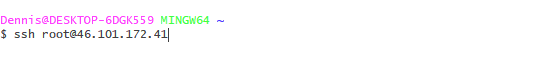
\includegraphics[width=1\textwidth]{../images/ssh1.png}
		\item It will prompt for the password
		\newline
		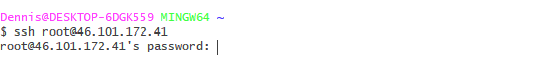
\includegraphics[width=1\textwidth]{../images/ssh2.png}
	\end{itemize}
	On successful login, connection to the remote server will be established and we can configure the server as per our requirements.
	\subsection*{Transferring files to remote servers}
	There are two ways in which we can transfer our files to the remote servers. One is by using Git and the other is a file transfer software called Filezilla.
	
	\subsection*{Git}
	Git, a distributed version control system that syncs repositories across different machines and Github to track code remotely. Creating a git repository is relatively easy. In this project, the Node remote server is setup using Git. In order to transfer files from a local machine, it needs to be located inside a directory with git initialized and synced with Github. This can be done by running the following command in the terminal -
	\begin{verbatim}
	git init
	\end{verbatim}
	
	This command creates a git repository, with a .git directory with subdirectories for objects, refs/tags, refs/heads, template files etc. Now, any change that is made inside the directory is watched by git. It maintains a compared list between new versions and old version of the directory. The command 'git status' gives us the current status of the directory compared to the previous saved state.
	\newline
	
	In order to sync new changes to the repository, the command 'git commit' is used. A commit is a record of what files have been changed since the last commit or initial commit(git init). Commits help us to control the state of our code allowing us to rollback to a certain commit if required.
	\newline
	
	For the purpose of sharing code between the local and remote servers, Github enables developers to do so. By uploading the local git repository to Github we can share our code. This is done in the following way -
	\begin{itemize}
		\item First we add a remote git repository, this is done in the following way - 
		\begin{verbatim}
		git remote add origin https://github.com/username/repositoryname.git
		\end{verbatim}
		This tells the local git repository to sync with the remote repository on Github located in the specified URL.
		\smallskip
		\item Once the remote repository is saved, push the current local repository and all it's files to the Github repository -
		\begin{verbatim}
		git push -u origin branchname
		\end{verbatim}
		origin indicates the remote repository to push to and branchname is the branch we wish to upload.
		\smallskip
		\item The code is now available on the remote Github repository and can be shared with any other computer.
	\end{itemize}
	Once the code is uploaded to the remote Github repository, it is time to download the code into the remote server.
	\begin{itemize}
		\item Login to the remote server via SSH using the appropriate IP address, username and password.
		\smallskip
		\item In order to clone the repository into our remote server machine, we use the 'git clone' command
		\begin{verbatim}
		git clone https://github.com/username/repositoryname.git
		\end{verbatim}
		This clones the git repository into the directory in the remote server. Now we can use the code the same way we did in the local machine.
	\end{itemize}
	\subsection*{Filezilla}
	Filezilla is a cross-platform FTP, SFTP and FTPS client with an intuitive graphical user interface. It allows transfer of files from one machine to another view the file transfer protocol. The server files for PHP and Django are transferred to their respective remote servers using the Filezilla client.
	\newline
	
	The main features of Filezilla are:
	\begin{itemize}
		\item Allows transfer of files in FTP, SFTP and also encrypted protocols of FTPS and SFTP
		\smallskip
		\item Supports IPv6, the latest internet protocol version
		\smallskip
		\item Directory comparison to compare local files and server files within the same directory. It also provides highlighting of missing or mismatched files
		\smallskip
		\item Ability to configure network settings
		\smallskip
		\item Support for remote file editing
		\smallskip
		\item HTTP/1.1, SOCKS5 and FTP-Proxy support
	\end{itemize}

	Compared to git, transferring files via Filezilla is relatively easier and quicker to achieve. The user can directly login to the remote server within Filezilla using the IP address, username and password of the remote server, on success browse the directories in the server and make file transfers.
	\subsection{Testing tool}
	Apachebench is used to load test both the local and the remote servers. It provides most of the key metrics required to make our comparison of the performance of the various web technologies discussed in this project. The nature of benchmark testing is http based and Apachebench provides the functionalities of making requests with multiple users as well as with concurrency. Apachebench generates a flood of queries to the specified URL and returns a variety of metrics. These metrics can be used to compare the performance of various web technologies in our project. Some of the important metrics are requests/second, time per request, and transfer rate. The tool allows testers to load test a URL or server by replicating number of users and number of concurrent requests per second.
	\newline
	
	Apachebench comes bundled with the XAMPP installation required for PHP. In order to run Apachebench we need to navigate to the folder /xampp/apache/bin where the ab.exe file is located. Next, we load up the terminal and execute the command 
	\begin{verbatim}
	ab -n numberOfUsers -c concurrency http://siteToBenchmark.com/
	\end{verbatim}
	where numberOfUsers is an integer value which takes the number of users to benchmark the URL with and concurrency indicates the number of simultaneous users making the request to the server.
\end{document}